\def\year{2021}\relax
%File: formatting-instruction.tex
\documentclass[letterpaper]{article} % DO NOT CHANGE THIS
\usepackage{aaai20}  % DO NOT CHANGE THIS
\usepackage{times}  % DO NOT CHANGE THIS
\usepackage{helvet} % DO NOT CHANGE THIS
\usepackage{courier}  % DO NOT CHANGE THIS
\usepackage[hyphens]{url}  % DO NOT CHANGE THIS
\usepackage{graphicx} % DO NOT CHANGE THIS
\urlstyle{rm} % DO NOT CHANGE THIS
\def\UrlFont{\rm}  % DO NOT CHANGE THIS

\usepackage{amssymb,amsmath,bm}
\usepackage{graphics,adjustbox}
\usepackage{tikz}
\usepackage{subcaption}
\usepackage{float}
\usepackage{siunitx}
\sisetup{unitsep = \cdot}

\usepackage[figuresright]{rotating}
\usepackage[colorinlistoftodos]{todonotes}
\usepackage[english,algo2e,algoruled,vlined,linesnumbered]{algorithm2e}   % package for algorithm
\usepackage{enumerate}

\usepackage{easyReview}
\newtheorem{assumption}{Assumption}


\DeclareMathOperator*{\argmin}{arg min}


\frenchspacing  % DO NOT CHANGE THIS
\setlength{\pdfpagewidth}{8.5in}  % DO NOT CHANGE THIS
\setlength{\pdfpageheight}{11in}  % DO NOT CHANGE THIS
%\nocopyright
%PDF Info Is REQUIRED.
% For /Author, add all authors within the parentheses, separated by commas. No accents or commands.
% For /Title, add Title in Mixed Case. No accents or commands. Retain the parentheses.
 \pdfinfo{
/Title (Smart Sanitizing Indoor Mobile Robot: Design and Development)
/Author (Brian Lauer, Nicoulas Shepard, Fazel Keshtkar, and Md Suruz Miah)
} %Leave this	
% /Title ()
% Put your actual complete title (no codes, scripts, shortcuts, or LaTeX commands) within the parentheses in mixed case
% Leave the space between \Title and the beginning parenthesis alone
% /Author ()
% Put your actual complete list of authors (no codes, scripts, shortcuts, or LaTeX commands) within the parentheses in mixed case. 
% Each author should be only by a comma. If the name contains accents, remove them. If there are any LaTeX commands, 
% remove them. 

% DISALLOWED PACKAGES
% \usepackage{authblk} -- This package is specifically forbidden
% \usepackage{balance} -- This package is specifically forbidden
% \usepackage{caption} -- This package is specifically forbidden
% \usepackage{color (if used in text)
% \usepackage{CJK} -- This package is specifically forbidden
% \usepackage{float} -- This package is specifically forbidden
% \usepackage{flushend} -- This package is specifically forbidden
% \usepackage{fontenc} -- This package is specifically forbidden
% \usepackage{fullpage} -- This package is specifically forbidden
% \usepackage{geometry} -- This package is specifically forbidden
% \usepackage{grffile} -- This package is specifically forbidden
% \usepackage{hyperref} -- This package is specifically forbidden
% \usepackage{navigator} -- This package is specifically forbidden
% (or any other package that embeds links such as navigator or hyperref)
% \indentfirst} -- This package is specifically forbidden
% \layout} -- This package is specifically forbidden
% \multicol} -- This package is specifically forbidden
% \nameref} -- This package is specifically forbidden
% \natbib} -- This package is specifically forbidden -- use the following workaround:
% \usepackage{savetrees} -- This package is specifically forbidden
% \usepackage{setspace} -- This package is specifically forbidden
% \usepackage{stfloats} -- This package is specifically forbidden
% \usepackage{tabu} -- This package is specifically forbidden
% \usepackage{titlesec} -- This package is specifically forbidden
% \usepackage{tocbibind} -- This package is specifically forbidden
% \usepackage{ulem} -- This package is specifically forbidden
% \usepackage{wrapfig} -- This package is specifically forbidden
% DISALLOWED COMMANDS
% \nocopyright -- Your paper will not be published if you use this command
% \addtolength -- This command may not be used
% \balance -- This command may not be used
% \baselinestretch -- Your paper will not be published if you use this command
% \clearpage -- No page breaks of any kind may be used for the final version of your paper
% \columnsep -- This command may not be used
% \newpage -- No page breaks of any kind may be used for the final version of your paper
% \pagebreak -- No page breaks of any kind may be used for the final version of your paperr
% \pagestyle -- This command may not be used
% \tiny -- This is not an acceptable font size.
% \vspace{- -- No negative value may be used in proximity of a caption, figure, table, section, subsection, subsubsection, or reference
% \vskip{- -- No negative value may be used to alter spacing above or below a caption, figure, table, section, subsection, subsubsection, or reference

\setcounter{secnumdepth}{0} %May be changed to 1 or 2 if section numbers are desired.

% The file aaai20.sty is the style file for AAAI Press 
% proceedings, working notes, and technical reports.
%
\setlength\titlebox{2.5in} % If your paper contains an overfull \vbox too high warning at the beginning of the document, use this
% command to correct it. You may not alter the value below 2.5 in
\title{Smart Sanitizing Mobile Robot using Ultra-violet Sterilization
  Technology: A Prototype}
%Your title must be in mixed case, not sentence case. 
% That means all verbs (including short verbs like be, is, using,and go), 
% nouns, adverbs, adjectives should be capitalized, including both words in hyphenated terms, while
% articles, conjunctions, and prepositions are lower case unless they
% directly follow a colon or long dash
\author{~%
Brian Lauer\textsuperscript{\rm 1}, Nicoulas Shepard\textsuperscript{\rm 1},
Fazel Keshtkar\textsuperscript{\rm 2}, and Md Suruz Miah\textsuperscript{\rm 1}
\\  
\textsuperscript{\rm 1}Electrical and Computer Engineering, Bradley University, Peoria, IL, USA; emails:~\{blauer,nshepard\}@mail.bradley.edu,~smiah@bradley.edu\\
\textsuperscript{\rm 2}Computer Science, Math. and Science, St John's University, Queens, NY, USA; email:~keshtkaf@stjohns.edu
}
 \begin{document}

\maketitle

\begin{abstract}

  In this paper, we propose a design of a smart sanitizing wheeled mobile robot
  using ultra-violet (UV) sterilization technology. The current design of the
  robot includes exteroceptive sensors, such as sonars, a lidar, a radio-frequency
  transceiver, and a camera. A circular-shaped UV [wavelength is in the range of
  $200~\nano\meter$--$280~\nano\meter$ (C band)] LED light is mounted on top
  of the robot for the purpose of sterilization in sanitizing complex indoor
  environments. The proposed robot under development is expected to sanitize  
  complex environments smartly in the sense that the UV LED is mounted with an actuator so that the robot can
  easily adapt the height of the UV LED based on the map of the operating
  environment. The performance of the robot is
  initially tested using the commercial robot simulator in an indoor environment
  with various complexities.   

\end{abstract}

\section{Introduction}
\label{sec:introduction}

-The design and development of a class of mobile robots in sterilizing indoor
-environments, hospitals, offices, and other indoor spaces, for example, have
-received a special attention in recent years, especially due to Coronavirus
-diseases - 2019 (COVID-19)\todo[inline]{Reference}. Recently, a class of mobile robots has been
-developed to sterilize indoor spaces using UV-C sterilization
-technology~\todo[inline]{Reference}. Most of the mobile robots developed so far in
-sanitizing indoor environments either rely on fixed-mount UV-tube or sprayers to
-disinfect areas much like a conventional cleaning robot. It is worth noting
-that, not many sanitizing robots use UV lights to disinfect robot based on the
-map of the indoor operating environment. In this paper, we develop a prototype
-of a modular and cost-effective mobile robot, where robot has the ability to
-smartly decide on the indoor space to  be sterilize based on the map. The map of
-the environment is created using sensor fusion technology much like what
-conventional autonomous robots do using range and vision sensors.
\section{Existing Sanitizing Robots} 
\section{Existing Sanitizing Robots} 
\label{sec:Literature}
There are many ways of transmitting infections disease, and studies have shown that the greatest cause of contact surface such as: remote control, door handles or cabinets, a button to call for help, etc. UV-C disinfection robot provides an economical and effective measure in limiting the spread of bacteria.  UV-C disinfection robot provides an economical and effective measure in limiting the spread of bacteria. When bacteria are exposed to UV-C light of their DNA absorbs light energy and causes cell damage that prevents new infecting others. The robot is controlled by the medical staff and the time for which disinfect a room is 10–15 min depending on the size of the room. 

\subsubsection{Service Robots for Disinfection}
In their paper, \cite{Begic2018} investigated the use of of the service robots in medicine with an emphasis on service robots for disinfection in medical institutions. They found that  disinfectant service robots are fast and effective in medical institutions.  Most imprtant;y, they found that use of the service robots reduces the risk of infection, cost of traditional cleaning and disinfection, and most importantly acquires confidence and security in medical facilities. In their paper, they investigated following service robots:
\begin{itemize}
	\item \textbf{Robot 'IRIS 3200 m'}
	One of the UV light robot is \verb|IRIS 3200 m|, which  is the most powerful system for disinfecting UV light in the world. This robot   UVC generate UVC  up to 20 times the UVC output tested xenon pulse system and three times the power of other constant light competitors.
	This robot uses  patented SmartDosage, together with the patented box Balance and PowerBoost technology allow 'iris 320m' UV lighting system of disinfection for automatically measuring conditions the room environment, such as the size of the room, temperature and humidity in order to determine in real time the appropriate dose, time, number and power of the lamp is required for complete disinfection of all while providing maximum power permitted in the United States for the production of germicidal UVC energy.
	
	IRIS 3200 m is ideal for the hospital which require the maximum disinfection least amount of time. Benefits 'Iris 3200 m' UV light disinfection system are: Faster treatment room, Higher productivity, More effective treatments, Highly pathogenic kills prices, Whole-room treatments, One placement, One treatment
	
	\item "Xenex Germ-Zapping" Robots
	High intensity ultraviolet light is produced by xenon flash lamps across the entire disinfecting spectrum known as UV-C. This UV-C energy passes through the cell walls of bacteria, viruses and bacterial spores. The DNA, RNA and proteins inside the microorganism absorb this intense UV-C energy. Xenex Full Spectrum UV-C provides four mechanisms of damage against pathogens. 
	The primary types of cellular damage caused by Pulsed Xenon UV are photohydration (pulling water molecules into the DNA that prevents transcription), photosplitting (breaking the backbone of the DNA), and photodimerization (improper fusing of DNA bases), all of which prevent cell replication.
\end{itemize}

\subsubsection{Wall-Following Behavior for a Disinfection Robot Using Type 1 and Type 2 Fuzzy Logic Systems}
% https://pubmed.ncbi.nlm.nih.gov/32784888/
\cite{Muthugaletal2020} 
Robot-aided solutions are demanded to disinfect possibly contaminated surfaces to reduce the spread of infectious diseases. A wall disinfection robot should be capable of following a given wall while maintaining a specified distance from the wall. The ability to maintain the specified distance from the wall is crucial for the effective sterilization of the wall surface since the intensity of the disinfectant agent applied on the wall depends on the distance. The disinfectant agent can be either a sprayable liquid, a gas, or ultraviolet light directed at the wall. Therefore, this paper proposed a novel method to establish the wall-following behavior for a disinfection robot.
The proposed method was designed in such a way that it enables a robot to follow a wall of an unknown environment by online path planning based on the range sensor information. Fuzzy logic was used for establishing the wall-following behavior based on the range sensor inputs. A Type 1 Fuzzy Logic System (T1-FLS) and an Interval Type 2 Fuzzy Logic System (IT2-FLS) were proposed in this regard. The FLSs were designed in such a way that they were generalized from the lateral distance to be maintained from a wall. Moreover, users can alter the lateral distance per the requirements without performing any redesign work of the system. The FLSs take the information perceived from range sensors as inputs and determine the linear velocity and the angular velocity of the robot required to follow a wall successfully.
Simulations were conducted to evaluate the characteristics and performance of the proposed FLSs. Heterogeneous test cases that consisted of typical wall arrangements were considered in the simulation. According to the simulation results, both proposed FLSs (i.e., T1-FLS and IT2-FLS) were capable of adequately following walls as expected for a wall disinfection robot. A superior performance could be observed from the IT2-FLS compared to that of the T1-FLS, and this performance difference was large and statistically significant. The real-world applicability of the proposed method was verified from the simulations, and it is expected that real-world trials will be conducted in the next phase of the work.

\subsubsection{UVC disinfection robot}
%https://www.ncbi.nlm.nih.gov/pmc/articles/PMC7556603/

\cite{Guettari2020} The aim of the present work is to contribute in the fight against the spread of Covid-19, a novel human coronavirus, in hospitals, public transport, airlines, and any enclosed areas. They have adopted the physical disinfection method by using UVC light as agent. The UVC devices are studied and classified according their disinfectant units, complementary devices, combined disinfection agents, mobilities, and order types. Their finding shows that a mobile robot is the most efficient device to inactivate microorganisms, so they have developed a robot called 'i-Robot UVC'. The robot is equipped with eight UVC lamps around a central column and two lamps on the top. 
i-Robot UVC can be controlled manually or run automatically; the robot is designed especially for all areas of hospital and any enclosed space to inactivate microorganisms. The construction of the robot involved: (1) the structural building, (2) the electronic assembling, and (3) the programming of the microcontroller and the mobile application.
The structure was made by attaching to a central column two horizontal crows to immobilize eight UVC lamps. Two other lamps are mounted on top of the robot; the system of lamps can cover the space around the device. The power supply of the device is done with a direct voltage of 24 V which supplies energy to the UVC lamps and supplies the Arduino board and the rest of the electronic circuit.

Some features of i-Robot UVC:   disinfectant time is estimation based on space,  the temperature, and the humidity rate; uses ultrasound sensor to detect and measure the distance; Using infrared sensors  to detect motion;  robot operates when people are not around and turns off the UVC lamps otherwise; using  to LiDAR sensor, the robot scans the environment and creates a digital map; this permits to optimize intervention. An operator equipped by protective suit controls the robot operation from a dashboard thanks to integrated cameras.



\section{System Architecture}
\label{sec:SystemArchitecture}

\todo[inline]{Discuss two different architecture that we propose}

\begin{figure}[htpb]
  \centering
  \begin{subfigure}[b]{0.5\textwidth}
    \centering
    \includegraphics[scale=0.25]{../figs/img/frontViewScreenshotB}
    \caption{Overall design of the proposed smart sanitizing robot.}
    \label{fig:frontViewScreenshotB}
  \end{subfigure}
  \begin{subfigure}[b]{.5\textwidth}
    \centering
    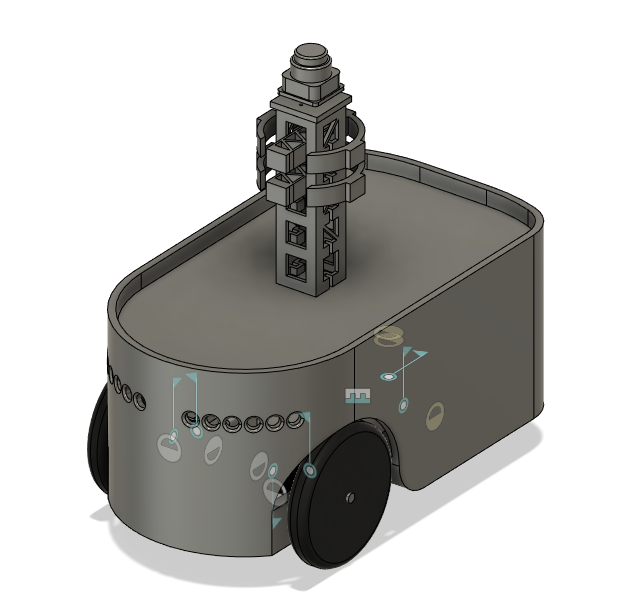
\includegraphics[scale=0.3]{../figs/img/v3BodyDesign}
    \caption{Body design}
  \end{subfigure}
  \begin{subfigure}[b]{.5\textwidth}
  	\centering
  	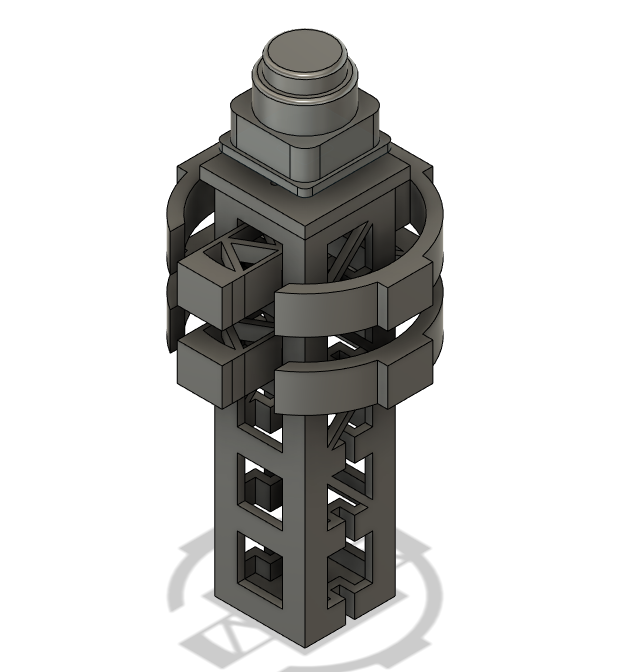
\includegraphics[scale=0.3]{../figs/img/lidarTowerFinal}
  	\subcaption{Lidar tower model}
  \end{subfigure}

  \caption{Design of Proposed Sanitizing Robots.}
  \label{fig:ArchitecturesOfSanitizingRobot}
\end{figure}


\subsection{Features}
\label{sec:Features}

\subsection{Operating Principle}
\label{sec:OperatingPrinciple}



\section{Detailed Design}
\label{sec:DetailedDesign}



\section{Real-Time Computer Experiment}
\label{sec:RealTimeComputerExperiment}
The proposed robot design was simulated in the commercial robot simulator known as Coppelia Sim. 
\begin{figure}[H]
\centering
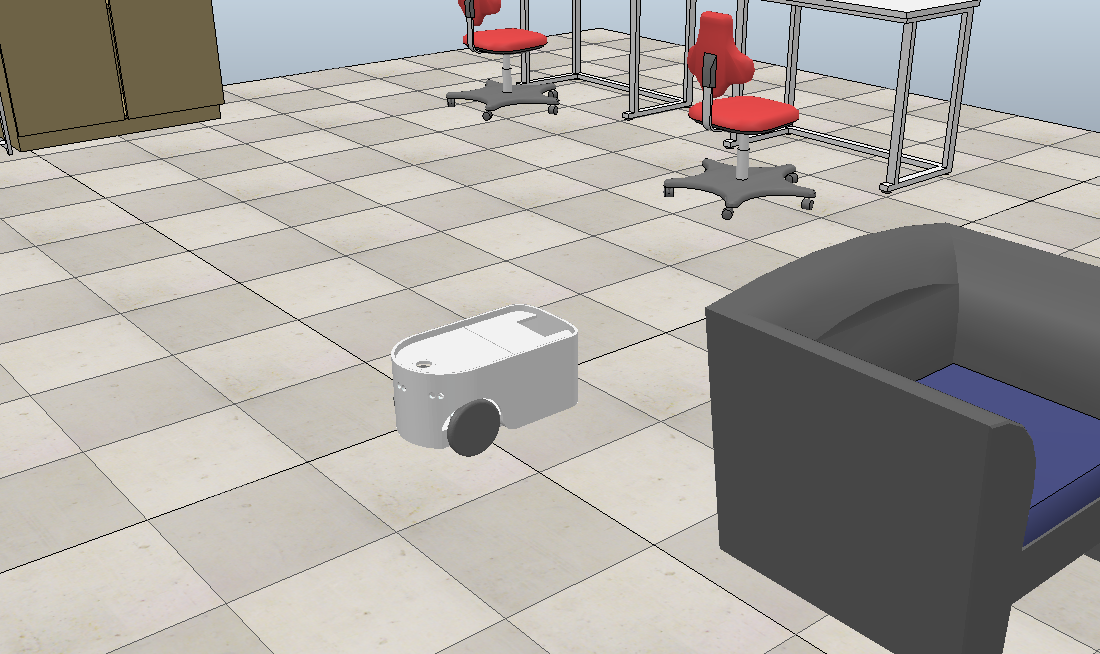
\includegraphics[scale=0.2]{../figs/img/copSimCap}
\caption{CoppeliaSim simulation of the proposed robot}
\end{figure}

\section{Conclusion}
\label{sec:conclusion}


 \bibliographystyle{aaai}
 \bibliography{bib/flairs34}
 %{bib/refsSuruzWeb,bib/refsMultiAgent,bib/refsRoboticsJournals,bib/refsRoboticsConferences,bib/refsGenericControl,bib/refsBooksTRTheses,bib/refsReinforcementLearningADP,bib/refsRL-Keshtkar}

\end{document}

%%% Local Variables:
%%% mode: latex
%%% TeX-master: t
%%% End:
